\section{Equivalent transformer}
\subsection{Circuit diagram}
\begin{figure}[H]
    \centering
    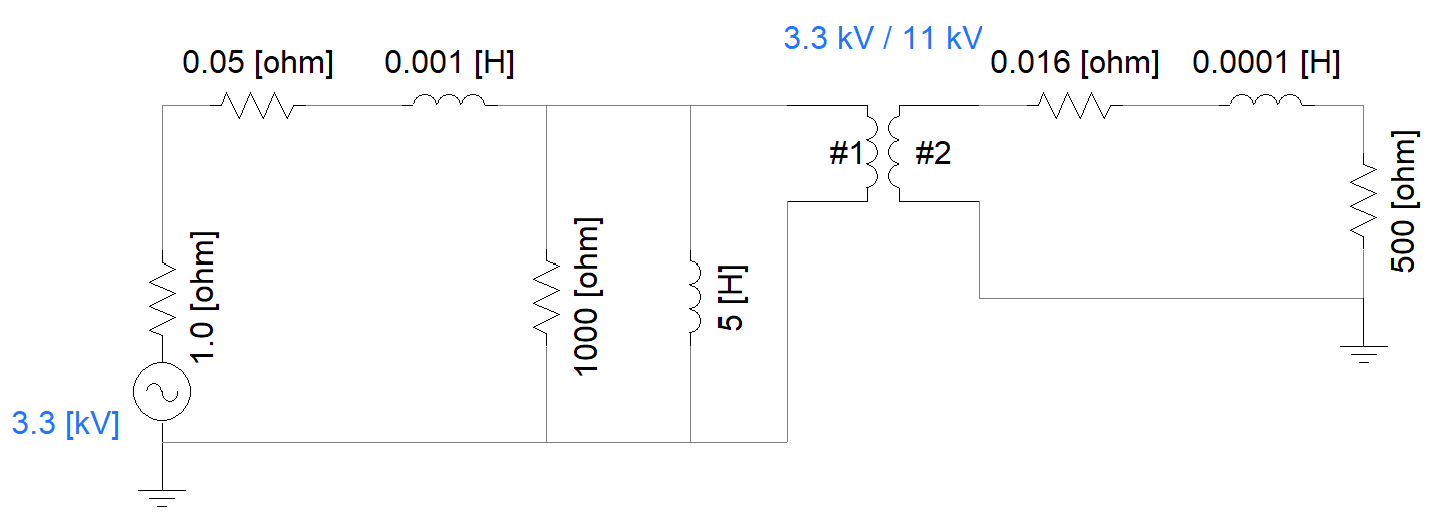
\includegraphics[width = \textwidth]{img/figure5.png}
    \caption{Circuit diagram to show equivalent transformer.}
    \label{fig:transformerCircuit}
\end{figure}
\subsection{Resistive load}
MATLAB code for this section of the assignment can be viewed in Appendix \ref{app:q2}.
\subsubsection{RMS Voltage }
The RMS voltage can be calculated using \eqref{VRMS}.
\begin{gather}\label{VRMS}
    V_{RMS} = \sqrt{\dfrac{\sum_{i=1}^n x_i^2}{n}}
\end{gather}
\begin{itemize}
    \item Simulation time: \SI{0.5}{\second}
    \item Number of data points ($n$): 2002
\end{itemize}
Using MATLAB, the RMS voltage over the time period is:
\begin{gather}
    V_{RMS,r} = \SI{10.14}{\kilo\volt}
\end{gather}
\begin{figure}[H]
    \centering
    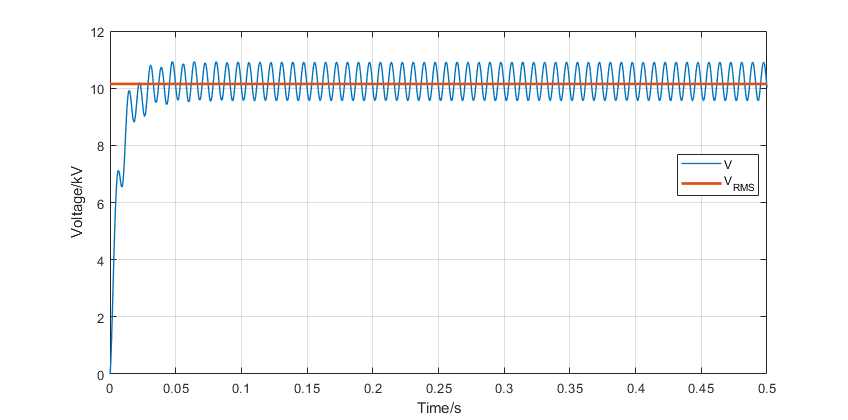
\includegraphics[width = 0.75\textwidth]{img/figure8.png}
    \caption{Voltage across load over time and value of $V_{RMS,r}$ for the time period.}
    \label{fig:VRMSResistor}
\end{figure}
\subsubsection{Power factor}
The power factor can be calculated using the following equation:
\begin{gather}
    PF = \cos \phi
\end{gather}
Using MATLAB, the converged value of the power factor was found by averaging the final values in the dataset.
\begin{gather}
    PF_{r} = 0.995
\end{gather}
\begin{figure}[H]
    \centering
    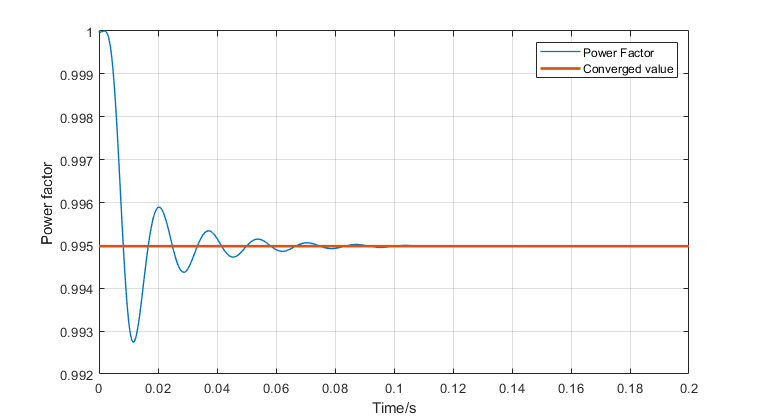
\includegraphics[width = 0.75\textwidth]{img/figure6.png}
    \caption{Power factor over time (resistor).}
    \label{fig:PFResistor}
\end{figure}
\subsection{Inductive load}
\subsubsection{RMS Voltage}
Using MATLAB, the RMS voltage over the time period is:
\begin{gather}
    V_{RMS,i} = \SI{2.79}{\kilo\volt}
\end{gather}
\begin{figure}[H]
    \centering
    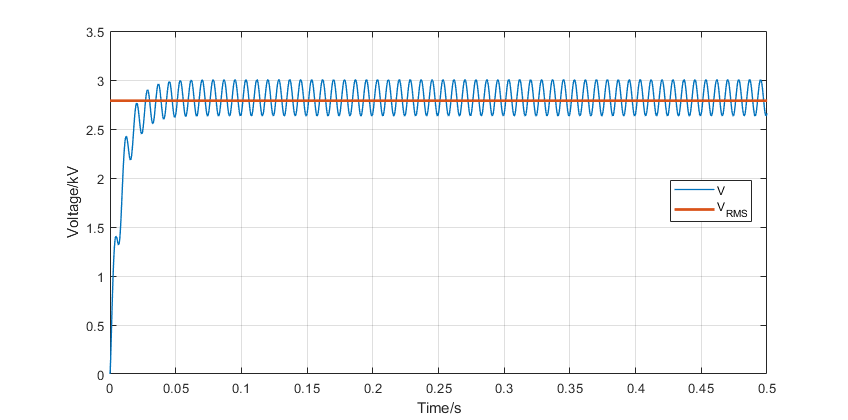
\includegraphics[width = 0.75\textwidth]{img/figure7.png}
    \caption{Voltage across load over time and value of $V_{RMS,i}$ for the time period.}
    \label{fig:VRMSInductor}
\end{figure}
\subsubsection{Power factor}
Using MATLAB:
\begin{gather}
    PF_{i} = 0.563
\end{gather}
\begin{figure}[H]
    \centering
    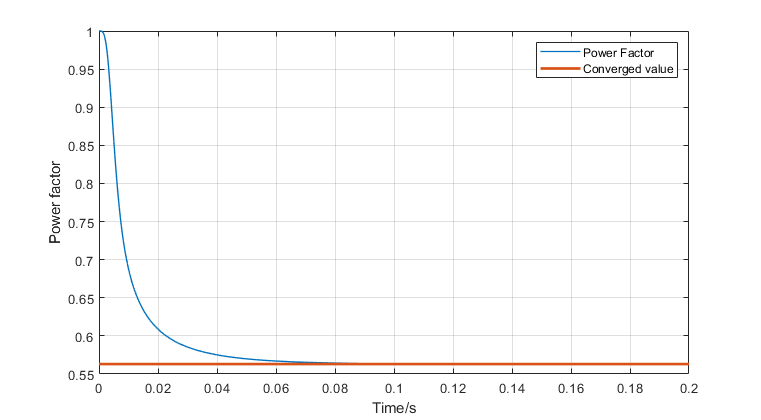
\includegraphics[width = 0.75\textwidth]{img/figure10.png}
    \caption{Power factor over time (inductor).}
    \label{fig:PFInductor}
\end{figure}
\subsection{Capacitive load}
\subsubsection{RMS Voltage}
Using MATLAB, the RMS voltage over the time period is:
\begin{gather}
    V_{RMS,c} = \SI{0.262}{\kilo\volt}
\end{gather}
\begin{figure}[H]
    \centering
    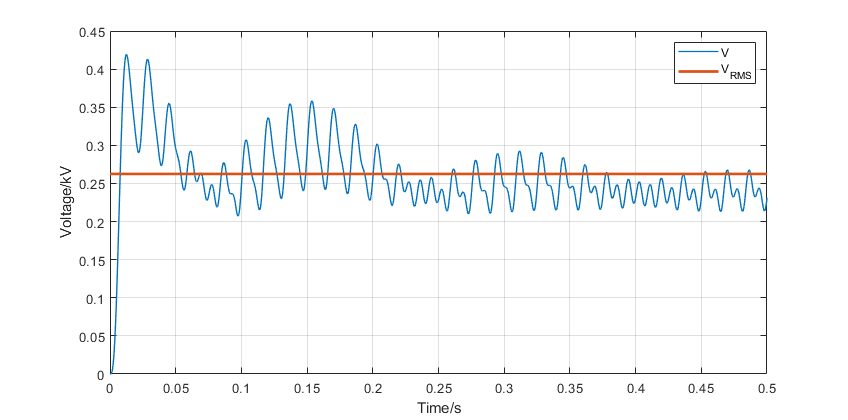
\includegraphics[width = 0.75\textwidth]{img/figure9.png}
    \caption{Voltage across load over time and value of $V_{RMS,c}$ for the time period.}
    \label{fig:VRMSCapacitor}
\end{figure}
\subsubsection{Power factor}
Using MATLAB:
\begin{gather}
    PF_{c} = -0.328
\end{gather}
\begin{figure}[H]
    \centering
    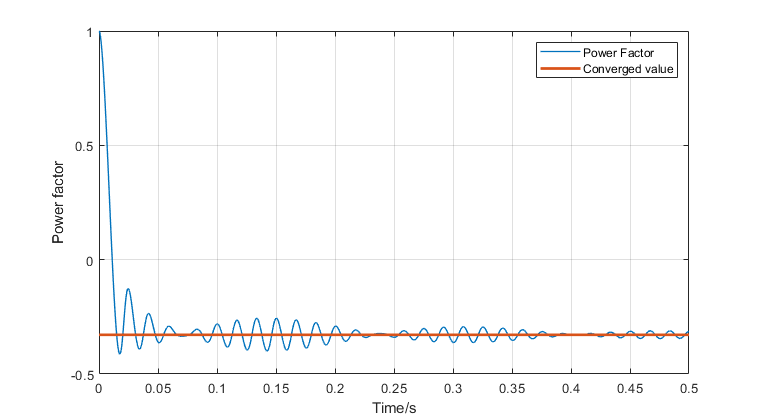
\includegraphics[width = 0.75\textwidth]{img/figure11.png}
    \caption{Power factor over time (capacitor).}
    \label{fig:PFCapacitor}
\end{figure}